\chapter{Implementatie}
\label{ch:implementation}
Dan is het nu tijd om onze POC te implementeren met de technologieën die hierboven besproken zijn.
Hieronder wordt gepoogd om zo specifiek mogelijk uit te leggen wat de verschillende ontwikkelingsstappen zijn en wat de manier is waarop deze zijn geïmplementeerd.

Dit project is geforked van chat-langchain, een voorbeeldimplementatie gebruikt door langchain om te chatten met hun developerdocumentatie.
Langchain host dit normaliter in de cloud, dus is er wat aanpassingswerk nodig om ervoor te zorgen dat alles veilig lokaal draait in een gecontroleerde omgeving.

\section{Writeup: Backend}
Deze sectie handelt over het instellen van het LangChain en Ollama systeem en het in staat te stellen om met FastAPI te communiceren met onze NextJS frontend.

\subsection{Geïnstalleerde software}
Vooraleerst hebben we een selectie aan software nodig om alles lokaal te kunnen draaien:
\begin{itemize}
	\item \textbf{Docker + compose plugin}
	\item \textbf{Python3 + pipx + poetry venv manager}
	\item \textbf{Ollama}
	\item \textbf{Embeddings model: nomic-embed-text}
	\item \textbf{Large-language-model: mistral}
	\item \textbf{Chroma}
	\item \textbf{PostgreSQL}
\end{itemize}

Chroma kan gecloned worden via \url{git@github.com:chroma-core/chroma.git} en gerund worden via \lstinline{docker compose up -d --build} in de geclonede directory. \\
Postgres kan gepulled worden van docker hub via \lstinline{docker pull postgres} en gerund worden via \lstinline{docker run -d --name postgres -e POSTGRES\_PASSWORD=root postgres} . \\

Als alles goed draait en als je een list command runt voor docker zal er een gelijkaardige output verschijnen zoals onderstaande screenshot:
\begin{figure}[h]
	\makebox[\textwidth]{
		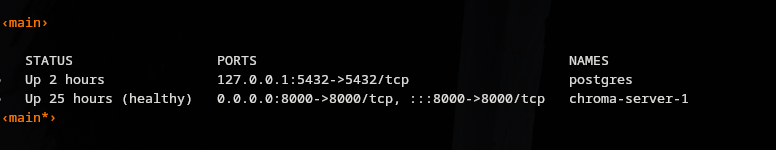
\includegraphics[width=\textwidth]{docker_containers.png}
	}
\end{figure}

Ollama kan geïnstalleerd worden via hun site \url{https://ollama.com} en dan via een command prompt kan je de modellen downloaden: \lstinline{ollama pull nomic-embed-text \&\& ollama pull mistral}. \\

Alle andere packages zijn normaal beschikbaar uit de package repositories van alle populaire distributies.

\subsection{Opzetten van lokale omgeving}
Allereerst zullen we het project importeren dat we zullen aanpassen, dit kan gecloned worden via \lstinline{git clone --branch langserve --single-branch https://github.com/langchain-ai/chat-langchain/}.
Daarna installeren we alle packages in onze repository via \lstinline{poetry install}. Dit creëert een virtuele python omgeving. Installeer ook de pypdf module via \lstinline{poetry add pypdf}.
Virtuele python omgevingen zijn handig als je geen dependency hell wilt veroorzaken met meerdere projecten op dezelfde machine. \\

Nu hebben we nog documenten nodig.
Er zijn een aantal documenten van Deltalex verkregen en samen met een paar publieke wetboeken (om de schrijfstijl en het vocabularium van een advocaat na te bootsen) geplaatst in een directory.
Deze documenten verschillen van brieven, mails tot ingebrekestellingen en worden puur ter referentie gebruikt.

\subsection{Instellen van vectorstore en record store - ingest script}
Nu we alles hebben opgezet is het nog nodig om ons ingest script wat aan te passen om puur lokaal te draaien. Hierna volgt de implementatie gebruikt voor ons POC:
\newpage

\begin{lstlisting}
import logging
import os

from chromadb import HttpClient
from chromadb.config import Settings
from langchain.text_splitter import RecursiveCharacterTextSplitter
from langchain_core.embeddings import Embeddings
from langchain_chroma import Chroma
from langchain.indexes import SQLRecordManager, index
from langchain_community.embeddings.ollama import OllamaEmbeddings
from langchain_community.document_loaders import PyPDFDirectoryLoader
# add pypdf module to venv


logging.basicConfig(level=logging.INFO)
logger = logging.getLogger(__name__)


def get_embeddings_model() -> Embeddings:
    return OllamaEmbeddings(model="nomic-embed-text:latest")


def load_deltalex_pdfset():
    return PyPDFDirectoryLoader("/home/laurent/Documents/schoolrepos/HoGent1/bachelorsAssignment/deltalexDocs/").load()


def getChromaClient():
    return HttpClient(settings=Settings(anonymized_telemetry=False))


def ingest_docs():
    DATABASE_HOST = os.environ["DATABASE_HOST"]
    DATABASE_PORT = os.environ["DATABASE_PORT"]
    DATABASE_USERNAME = os.environ["DATABASE_USERNAME"]
    DATABASE_PASSWORD = os.environ["DATABASE_PASSWORD"]
    DATABASE_NAME = os.environ["DATABASE_NAME"]
    RECORD_MANAGER_DB_URL = f"postgresql://{DATABASE_USERNAME}:{DATABASE_PASSWORD}@{DATABASE_HOST}:{DATABASE_PORT}/{DATABASE_NAME}"
    COLLECTION_NAME = os.environ["COLLECTION_NAME"]

    vectorstore = Chroma(
        collection_name=COLLECTION_NAME,
        embedding_function=get_embeddings_model(),
        persist_directory="./deltalex_chroma",
        client=getChromaClient()
    )

    text_splitter = RecursiveCharacterTextSplitter(chunk_size=224, chunk_overlap=32)

    record_manager = SQLRecordManager(
        namespace="deltalex",
        db_url=RECORD_MANAGER_DB_URL
    )
    record_manager.create_schema()

    docs_transformed = text_splitter.split_documents(load_deltalex_pdfset())
    logger.info("docs transformed")

    indexing_stats = index(
        docs_transformed,
        record_manager,
        vectorstore,
        cleanup="full",
        source_id_key="source"
    )

    logger.info(indexing_stats)
    logger.info("docs added to vector database")


if __name__ == "__main__":
    ingest_docs()

\end{lstlisting}
Deze implementatie heeft een groot aantal verschillen van de originele github code. Allereerst worden er documenten uitgelezen uit een specifieke map naar mijn keuze.
Vervolgens worden ze gesplit in chunks tekst (van in totaal 256 karakters en wat overloop ingerekend) om dan doorgestuurd te worden naar een lokale Ollama instantie,
die ze transformeert naar vectoren in toevoegt in de database. \\

De volledige implementatie is lokaal en zal het netwerk van de machine niet verlaten.
De connectiestrings voor PostgreSQL worden uitgelezen uit environment variables.
De parameters voor een default chroma \lstinline{HttpClient} komen overeen met de settings van een docker compose container.
Een extra parameter voor anonymized telemetry zorgt ervoor dat er geen anonieme statistieken naar Chroma verstuurd worden. \\

Hier wordt ook voor het \lstinline{nomic-embed-text} model gekozen via OllamaEmbeddings.
Dat is een voorbeeld van een third party plugin van LangChain.

Het is de bedoeling dat dit script als eerst wordt gerund. Zonder vector store zal Deltalex Chat ook werken, maar zal er weinig relevante info gegeven worden door mistral alleen.
Als dit allemaal gerund heeft, is onze vectorstore klaar voor RAG gebruik.

\newpage
\subsection{Instellen van LLM en centraal systeem - Configureren van Langchain backend chain script}
\subsubsection{Aanpassing retriever}

Nu is het tijd om het systeem zelf te configureren. Veel van dit werk is al geïmplementeerd dankzij LangChain en de repo waarvan we gecloned hebben.
Deze klasse zorgt voor de interne afhandeling van requests aan ons systeem en is dus van elementair belang. \\ 

Dit systeem komt met een API voor later met onze frontend te communiceren en ook met een playground om prompts te testen en te zien wat er gebeurt achter de schermen. 
Het is eigenlijk de bedoeling om LangChain in de cloud te deployen (omdat cloud computers veelal sterkere grafische kaarten hebben en dus betere resultaten leveren)
maar via de tweaks die we nu maken is het mogelijk dit systeem volledig lokaal te draaien.\\

Allereerst passen we de vectorstore client weer aan naar Chroma en returnen we deze als vector retriever.
Deze functie zal dus verantwoordelijk zijn om relevante vectoren te retrieven en te gebruiken als context in het antwoord van onze LLM.
Dit is de functie in kwestie:

\begin{lstlisting}
def getChromaClient():
    return HttpClient(settings=Settings(anonymized_telemetry=False))


def get_retriever() -> BaseRetriever:
    vectorstore = Chroma(
        collection_name="deltalex",
        embedding_function=OllamaEmbeddings(model="nomic-embed-text:latest"),
        persist_directory="./deltalex_chroma",
        client=getChromaClient()
    )
    return vectorstore.as_retriever(search_kwargs=dict(k=6))

\end{lstlisting}

\newpage
\subsubsection{Prompt template}
Nu onze retriever is aangepast, is het ook heel belangrijk om een passend prompt template te maken voor onze Deltalex Chat.
Prompt templates zijn de wrapper rond LLM's. Een large language model heeft meestal een heel specifieke set instructies nodig om
naar behoren te functioneren. Deze prompt templates zijn ook wat een model de menselijke touch geeft.
Een voorbeeld van het gebruikte prompt template voor Deltalex Chat:

\begin{lstlisting}
    You are a lawyer, specialized in drafting legal documents for a Belgian law firm.
    From here on you write in Dutch. 
    This text from the context html tags is for linguistic purposes and to mimic a legal writing style. 
    
    Write a legal document, based on the provided context. 
    Use a professional and formal tone, suitable for a legal context. 
    
    Your writing style must be very formal and legal.
    Write in correct Dutch sentences and base yourself on the given documents inside the context html tags. 
    
    Anything between the following `context`  html blocks is retrieved from a set of legal documents.
    Use it as a linguistic reference. 
    You need to mimic the writing style to resemble that of a legal professional.
    
    <context> 
        {context}
    <context/>
    
    REMEMBER: 
    Do not write repetitive sentences. 
    Write in Dutch or French, based on the parameter given. Default will be Dutch. 
    Be very formal. 
\end{lstlisting}

De effectiviteit van een chatbot valt en staat met het prompt template. 
Het is niet simpel om een perfect template te fabriceren, maar gelukkig zijn er veel resources zoals \url{https://github.com/promptslab/Awesome-Prompt-Engineering?tab=readme-ov-file}
om ons daarmee te assisteren. \\

Dit is de laatste stap in het configuratieproces van het backend deel van onze implementatie. 

\newpage
\section{Frontend}
Deze sectie zal gaan over het aanpassen van de meegeleverde chat frontend naar onze wensen. 
Deze implementatie omvat een NextJS React project, gebouwd met ChakraUI en TailwindCSS. 

\subsection{Geïnstalleerde software}
Eerst installeren we best de software die we gaan gebruiken om het project te compileren. 
Dit korte lijstje omvat:

\begin{itemize}
    \item Node
    \item een node package manager zoals npm, pnpm, yarn, ... 
\end{itemize}

Deze tools zijn makkelijk te installeren uit de package managers van iedere populaire distributie. 

\subsection{Aanpassing van waarden}
